\documentclass[11pt,psfig]{article}
\usepackage{epsfig}
\usepackage{times}
\usepackage{amssymb}
\usepackage{float}

\newcount\refno\refno=1
\def\ref{\the\refno \global\advance\refno by 1}
\def\ux{\underline{x}}
\def\uw{\underline{w}}
\def\bw{\underline{w}}
\def\ut{\underline{\theta}}
\def\umu{\underline{\mu}} 
\def\bmu{\underline{\mu}} 
\def\be{p_e^*}
\newcount\eqnumber\eqnumber=1
\def\eq{\the \eqnumber \global\advance\eqnumber by 1}
\def\eqs{\eq}
\def\eqn{\eqno(\eq)}

 \pagestyle{empty}
\def\baselinestretch{1.1}
\topmargin1in \headsep0.3in
\topmargin0in \oddsidemargin0in \textwidth6.5in \textheight8.5in
\begin{document}
\setlength{\parskip}{1.2ex plus0.3ex minus 0.3ex}


\thispagestyle{empty} \pagestyle{myheadings} \markright{G}



\title{CS 266 Homework 2}
\author{Zachary DeStefano, PhD Student, 15247592}
\date{Due Date: April 17}

\maketitle

\vfill\eject

\subsection*{Problem 2.3}

Take the following line in FindNewEvent:
\begin{verbatim}
if $s_l$ and $s_r$ intersect below the sweep line, 
	or on it and to the right of the current event point p, 
	and the intersection is not yet present as an
	event in Q
\end{verbatim}
Modify it to make sure $s_l$ and $s_r$ are adjacent to each other before adding the intersection as an event. \\
\\
Storage:\\
This will ensure that only adjacent line segments are in the event queue, thus the storage is $O(n)$\\
\\
Correctness:\\
The segments will become adjacent again before an intersection point is reached, thus we do not have to worry about an intersection point not being reported with this modification. 

\newpage

\subsection*{Problem 2.11}

For this algorithm, we will split each circle into 4 quadrants and then test the intersections of all of the resulting arcs, ignoring the cases where it finds its own circle. Each arc will have a monotone x-coordinate and monotone y-coordinate, so we can take advantage of that property of line segments and thus use the FindIntersections code. \\
\\
Here is the algorithm:\\
\\
1. For each circle described by center $(a,b)$ and radius r, do the following:\\
- Make an arc that is the part of the circle where $a < x < a+r$ and $b < y < b+r$\\
- Make an arc that is the part of the circle where $a-r < x < a$ and $b < y < b+r$\\
- Make an arc that is the part of the circle where $a < x < a+r$ and $b-r < y < b$\\
- Make an arc that is the part of the circle where $a-r < x < a$ and $b-r < y < b$\\
Call the set of arcs found S\\
\\
2. Run FindIntersections(S) with the following changes\\
- In line 4 of HandleEventPoint(p), do not report the intersection if the two arcs are part of the same circle\\
- The FindNewEvent code stays the same, except that you should add both intersection points to the event queue in the case that there are two of them. \\
\\
Correctness:\\
The plane sweep algorithm will detect all the arcs and two arcs will become adjacent right before an intersection, thus the intersections will be detected. \\
\\
Running time:\\
The extra steps only add a constant number of operations, so it does not affect the big-Oh notation. \\
The run time of the algorithm is O($(n+I)logn$) in general.\\
In our case we have $4n$ arcs. \\
For number of intersections, there are at most $4n + k$ of them when you include the intersections of the quarter circles that are part of the same circle. \\
Thus our run time is bounded by 
\[
C(4n + (4n+k) )log(4n)
\]
for some constant C\\
This is still $O((n+k)logn)$

\newpage

\subsection*{Problem 8.4}

An intersection occurs when 
\[
x = \frac{b_2-b_1}{m_2-m_1}
\]
Thus if we take the minimum of $m_2-m_1$ and the maximum of $b_2-b_1$, we will get the maximum possible x coordinate of an intersection. If we do the same thing, but with inverse slope and y intercept, we will get the maximum possible y coordinate of an intersection. This fact will allow us to get a bounding box. We will later be able to get a tight bounding box.\\
\\
Here is algorithm for the initial bounding box:\\
1. Setup the following sets\\
		- Set B of y-intercepts of the lines\\
		- Set M of slopes of the lines\\
2. Compute the set $B*$ of x-intercepts of the lines. \\
			- for an individual $(m,b)$, this is equal to $-\frac{b}{m}$\\
3. Compute the set $M*$ of inverse slopes of the lines, meaning $1/m$. \\
4. Go through the set $B$ to get the min and max. Label them $b_{min}$ and $b_{max}$\\
5. Sort the set M and label the elements $m_1,...,m_n$ and put them in ascending order. \\
6. Find the min of $m_{i+1} - m_i$ for $1 \leq i \leq n-1$ and set it to $m'_{min}$ \\
7. Set $x_{max} = \frac{b_{max}-b_{min}}{m'_{min}}$\\
8. Set $x_{min} = -x_{max}$\\
9. Repeat steps 4-8 for $B*$ and $M*$ however in step 7-8, they will be $y_{max}$ and $y_{min}$. \\
10. The points $x_{min},x_{max},y_{min},y_{max}$ gives a bounding box\\
\\
Running time:\\
Step 1-4 all take O(n) time.\\
Step 5 will take O($n \, log n$) time. \\
Step 6 will take O(n) time. \\
The rest of the steps are constant time, except 9 which will be O($n log n$) time. \\
The total running time is thus O($n log n$) time. \\
\\
Correctness:\\
We showed above that the max possible difference in intercepts divided by the minimum possible difference in slopes gets the maximum x coordinate. The same argument will work with y coordinates. By the same token, if we make that fraction negative, then that is the minimum possible x coordinate and then y coordinate. Thus it is just left to prove that we have the min possible slope difference and the max possible intercept difference. For the min possible slope difference, we have to prove that the min difference between points on the number line is the min difference between adjacent numbers when they are sorted. For the max intercept difference, we have to prove that the max difference between points occurs as the difference between the max and the min. \\
\\
Proof of Max Difference: \\
Take sorted list $b_1,...,b_n$ which is in ascending order. \\Take any $1 \leq i,j \leq n$ where $i < j$. \\It suffices to show that $b_n - b_1 \geq b_j - b_i$. \\
This can be rearranged to $b_n-b_j \geq b_1-b_i$. \\
Since $b_n$ is the maximum, the left hand side is positive and since $b_1$ is the minimum, the right hand side is negative, thus the inequality holds. \\
\\
Proof of Min Difference: \\
Take the sorted list $m_1,...,m_n$ in ascending order.\\
Assume that for some $i < j < k$, the min difference in the set is $m_k-m_i$ however $m_j$ is between them. This means that $m_k-m_i \leq m_j-m_i$ which implies that $m_k \leq m_j$ which is a contradiction because this is a sorted list. \\
\\
Here is the algorithm to tighten the bounding box:\\
1. Take $y_{max}$ and compute the x-coordinates of the lines. \\
2. Sort the lines into $l_1,...,l_n$ by their x-coordinate at $y_{max}$. \\
3. For each adjacent pair of lines in the sorted list, $l_{i+1}$ and $l_i$\\
- Let $(x_i,y_i)$ be the intersection of $l_{i+1}$ and $l_i$\\
- Put the number $y_i$ into set $Y$\\
4. Set $y'_{max}$ to the max value of $Y$\\
5. Repeat steps 1-4 but for $y_{min}$ \\
- In Step 4, set $y'_{min}$ to be the min value of $Y$. \\
6. Repeat steps 1-5 but for the x coordinates\\
7. The tight bounding box is now $x'_{min}, x'_{max}, y'_{min}, y'_{max}$\\
\\
Running time:\\
All the steps except 2 and the repeats will take constant amount of time or O(n) time. \\
Step 2 will take O($n \, log n$) time for the sorting. \\
Computing the initial bounding box will take O($n \, log n$) time from above. \\
Thus the total running time is still O($n \, log n$). \\
\\
Correctness:
\\
WLOG, we will prove that the procedure is correct for getting the maximum y-value. \\
We already know that we have an upper bound for the maximum y vertex value. \\
It just suffices to prove that we only need to test adjacent lines at that upper bound. \\
Assume that we have three adjacent lines at that y-coordinate, $i < j < k$\\
We also have a case where the highest vertex is with the $(i,k)$ pair and not the $(i,j)$ pair or the $(j,k)$ pair \\
If we follow the $j$ line downward from the max y, which we can only do since the intersection cannot be above the max y, then because it is between $i$ and $k$, it must intersect either $i$ or $k$ before $(i,k)$ intersection. \\
At this intersection, there will be higher y-coordinate than the $(i,k)$ pair, a contradiction. 

\begin{figure}[H]
\centering
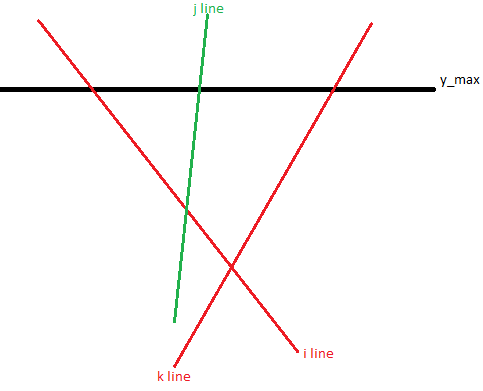
\includegraphics[height=3in]{hw2prob8_4_diagram.png}
\caption{The above argument with the $i,j,k$ lines illustrated}
\end{figure} 

\newpage

\subsection*{Problem 8.14}

Since a line through a pair of points in the primal plane becomes a vertex in the dual plane, we just have to compute the dual of the points and then compute which vertex has the most number of lines passing through it. \\
\\
Here is the algorithm:\\
1. Take the dual of the n points\\
2. Use the arrangement algorithm to find the vertices \\
3. Find which vertex contains the greatest number of lines \\
\\
Run time:\\
Taking the dual will take O(n) time \\
Computing the arrangement takes O($n^2$) time \\
Going through the vertices will take O($n^2$) time\\
The total running time is thus $O(n^2)$


%\begin{figure}[H]
%\centering
%\includegraphics[height=4in]{prob1plot.jpg}
%\caption{Probability of Class Labels with decision boundaries marked}
%\end{figure}


\end{document}








